% !TeX document-id = {81037089-d753-4843-b5ef-3370c781b644}
% !TeX spellcheck = en-US
% !TeX encoding = utf8
% !TeX program = pdflatex
% !BIB program = biber
% -*- coding:utf-8 mod:LaTeX -*-


\let\ifdeutsch\iffalse
\let\ifenglisch\iftrue
\input{pre-documentclass}
\documentclass[
  % fontsize=11pt is the standard
  a4paper,  % Standard format - only KOMAScript uses paper=a4 - https://tex.stackexchange.com/a/61044/9075
  twoside,  % we are optimizing for both screen and two-side printing. So the page numbers will jump, but the content is configured to stay in the middle (by using the geometry package)
  bibliography=totoc,
  %               idxtotoc,   %Index ins Inhaltsverzeichnis
  %               liststotoc, %List of X ins Inhaltsverzeichnis, mit liststotocnumbered werden die Abbildungsverzeichnisse nummeriert
  headsepline,
  cleardoublepage=empty,
  parskip=half,
  %               draft    % um zu sehen, wo noch nachgebessert werden muss - wichtig, da Bindungskorrektur mit drin
  draft=false
]{scrbook}
\input{config}


\usepackage[
  title={Reconceptualizing neural function as high-dimensional brain state dynamics},
  author={Adina S. Wagner},
  birth={aus Wolfsburg},
  type=doctoral,
  placeanddate={Düsseldorf, XXX 2023},
  institute={aus dem Institut für Experimentelle Psychologie\\der Heinrich Heine Universität Düsseldorf}, 
  reason={zur Erlangung des Doktorgrades
  	der Mathematisch-Naturwissenschaftlichen Fakultät
  	der Heinrich-Heine-Universität Düsseldorf},
]{scientific-thesis-cover}


% Hier stehen alle Abkürzungen
\newacronym{meg}{MEG}{magnetoencephalography}
\newacronym{rdm}{RDM}{Research data management}
\newacronym{er}{ER}{error rate}
\newacronym{fr}{FR}{Fehlerrate}
\newacronym[plural={RDBMS},shortplural={RDBMS}]{rdbms}{RDBMS}{Relational Database Management System}


\makeindex

\begin{document}

%tex4ht-Konvertierung verschönern
\iftex4ht
  % tell tex4ht to create picures also for formulas starting with '$'
  % WARNING: a tex4ht run now takes forever!
  \Configure{$}{\PicMath}{\EndPicMath}{}
  %$ % <- syntax highlighting fix for emacs
  \Css{body {text-align:justify;}}

  %conversion of .pdf to .png
  \Configure{graphics*}
  {pdf}
  {\Needs{"convert \csname Gin@base\endcsname.pdf
      \csname Gin@base\endcsname.png"}%
    \Picture[pict]{\csname Gin@base\endcsname.png}%
  }
\fi

%\VerbatimFootnotes %verbatim text in Fußnoten erlauben. Geht normalerweise nicht.

\input{commands}
\pagenumbering{arabic}
\Titelblatt

%Eigener Seitenstil fuer die Kurzfassung und das Inhaltsverzeichnis
\deftriplepagestyle{preamble}{}{}{}{}{}{\pagemark}
%Doku zu deftriplepagestyle: scrguide.pdf
\pagestyle{preamble}
\renewcommand*{\chapterpagestyle}{preamble}



\section*{Abstract}

Human brain mapping has focused on ascribing function to specific brain areas or networks.
But neural signals can be re-conceptualized from blobs of activity at any one time to dynamic and evolving trajectories through the high dimensional space spanned by the sensors that pick it up.
Over the last decade, this approach generated novel insights in the study of cognitive processes, and a variety of methods were formalized that build up on it, among them the shared response model.
In this work, the shared response model was used to study a cognitive process that has yet evaded our full understanding, namely that of working memory maintenance, the offline representation of information in absence of its original item.
Using magneto-encephalography data from a delayed decision making task, this work explored lower-dimensional subspaces of the high dimensional neural data to find latent factors representing fundamental trial properties during maintenance.
The analyses reveal ample evidence for preparatory decision signals during maintenance instead of decision-relevant stimulus properties, and establish the shared response model as a viable methodological choice for magneto-encephalic data.
However, the study of neural processes is not isolated from the social, organizational, and technical challenges underlying science.
Thus, this work further presents several projects in the area of research data management and research software engineering that laid foundational steps to enable trustworthy reusable project outcomes, from a software tool for data management and a community-based documentation effort to improve scientific conduct, to pragmatic strategies for research data management and the technical implementation of a scalable framework for reproducible data analysis.
While the findings on neural data for now only pertain to a single dataset and experiment, the technical solutions constitute widely reusable tools and methods for standard challenges in neuroscience and beyond.

%The growing digitization of research is accompanied by a steady and rapid growth in research data, and a sharp increase in the use of software \citep{dfg}

\pagebreak
\section*{Zusammenfassung}

Die Kartierung des menschlichen Gehirns hat sich darauf konzentriert, bestimmten Gehirnbereichen oder Gruppen funktional vernetzer Hirnareale eine Funktion zuzuordnen.
Eine alternative Betrachtungsweise ist es jedoch, neuronale Signale als dynamische und sich entwickelnde Trajektorien durch  hochdimensionale Signalräume zu rekonzeptualisieren.
In den letzten zehn Jahren hat dieser Ansatz zu neuen Erkenntnissen bei der Untersuchung kognitiver Prozesse geführt, und
eine Reihe neuartiger Methoden etabliert -- unter ihnen das Shared Response Model.
In der vorliegenden Arbeit wird das Shared Response Model genutzt, um einen kognitiven Prozess zu untersuchen, der sich bisher unserem vollständigen Verständnis entzogen hat: Die Aufrechterhaltung des Arbeitsgedächtnisses, d. h. die Bereithaltung von Informationen in Abwesenheit des ursprünglichen Reizes.
In dieser Arbeit wurden daher anhand von Magnetoenzephalographie-Aufnahmen eines Experiments zur verzögerten Entscheidungsfindung  niederdimensionale Unterräume der hochdimensionalen neuronalen Daten untersucht, um latente Faktoren zu finden, die  grundlegende Experimentcharakteristika im Arbeitsgedächtnis abbilden.
Die vorgestellten Datenanalysen liefern Belege dafür, dass vorbereitende Entscheidungssignale anstelle von entscheidungsrelevanten Stimuluscharakteristika im Arbeitsgedächtnis aufrecht erhalten werden, und etablieren das Shared-Response-Modell als anwendbar auf Magnetoenzephalographiedaten.
Analysen neuronaler Prozesse sind jedoch nicht von den sozialen, organisatorischen und technischen Herausforderungen wissenschaftlicher Projekte isoliert.
Daher werden in dieser Arbeit auch mehrere Projekte aus den \mbox{Bereichen} Forschungsdatenmanagement und Forschungssoftwareentwicklung vorgestellt, mit denen vertrauenswürdige, wiederverwendbare Forschungsresultate erstellt werden können -- von einem Softwaretool und einem Dokumentationsprojekt zur Verbesserung von Forschungsdatenmanagement bis hin zu pragmatischen Datenmanagementstrategien und der technischen Umsetzung eines skalierbaren computationalen frameworks für  reproduzierbare Datenanalysen.
Während sich die Erkenntnisse zum Arbeitsgedächtnis vorerst nur auf einen einzigen Datensatz und ein einziges Experiment beziehen, stellen die technischen Lösungen weithin wiederverwendbare Werkzeuge und Methoden für Standardaufgaben in den Neurowissenschaften und darüber hinaus dar.

\cleardoublepage


% BEGIN: Verzeichnisse

\iftex4ht
\else
  \microtypesetup{protrusion=false}
\fi

%%%
% Literaturverzeichnis ins TOC mit aufnehmen, aber nur wenn nichts anderes mehr hilft!
% \addcontentsline{toc}{chapter}{Literaturverzeichnis}
%
% oder zB
%\addcontentsline{toc}{section}{Abkürzungsverzeichnis}
%
%%%

%Produce table of contents
%
%In case you have trouble with headings reaching into the page numbers, enable the following three lines.
%Hint by http://golatex.de/inhaltsverzeichnis-schreibt-ueber-rand-t3106.html
%
%\makeatletter
%\renewcommand{\@pnumwidth}{2em}
%\makeatother
%

% chapters, sections, and subsections appear in the toctree
\setcounter{tocdepth}{2}
\tableofcontents

% Bei einem ungünstigen Seitenumbruch im Inhaltsverzeichnis, kann dieser mit
% \addtocontents{toc}{\protect\newpage}
% an der passenden Stelle im Fließtext erzwungen werden.

% include list of figures, tables, and listings as well as abbreviations without clear pages in-between
{\listoffigures\let\clearpage\relax\listoftables\let\clearpage\relax\listof{Listing}{List of Listings}\let\clearpage\relax\printnoidxglossaries}
%Wird nur bei Verwendung von der lstlisting-Umgebung mit dem "caption"-Parameter benoetigt
%\lstlistoflistings



%mittels \newfloat wurde die Algorithmus-Gleitumgebung definiert.
%Mit folgendem Befehl werden alle floats dieses Typs ausgegeben
%\listof{Algorithmus}{List of Algorithms}

%\listofalgorithms %Ist nur für Algorithmen, die mittels \begin{algorithm} umschlossen werden, nötig

\iftex4ht
\else
  %Optischen Randausgleich und Grauwertkorrektur wieder aktivieren
  \microtypesetup{protrusion=true}
\fi

% END: Verzeichnisse


% Headline and footline
%\renewcommand*{\pagestyle}{scrplain}
%\pagestyle{scrheadings}
%\pagestyle{scrheadings}
%\ihead[helloihead]{h}
%\chead[hellochead]{i}
%\ohead[holloohead]{\headmark}
%\cfoot[]{}
%\ofoot[\usekomafont{pagenumber}\thepage]{\usekomafont{pagenumber}\thepage}
%\ifoot[]{}


%%%%%%%%%%%%%%%%%%%%%%%%%%%%%%%%%%%%%%%%%%%%%%%%%%%%%%%%%%%%%%%%%%%%%%%%%%%%%%
%
% Embed all relevant content
%
%%%%%%%%%%%%%%%%%%%%%%%%%%%%%%%%%%%%%%%%%%%%%%%%%%%%%%%%%%%%%%%%%%%%%%%%%%%%%%


% !TeX root = ../main-english.tex
% !TeX spellcheck = en-US
% !TeX encoding = utf8
% -*- coding:utf-8 mod:LaTeX -*-

%This smart spell only works if no changes have been made to the chapter
%using the options proposed in preambel/chapterheads.tex.
\setchapterpreamble[u]{%
	\dictum[Albert Einstein]{We cannot solve our problems with the same level of thinking that created them}
}
\chapter{Introduction}
\label{chap:k1}

Look mom, some text!

\section{Brain state spaces}
This is an introduction into brain states and functional alignment
\pagebreak

\section{Magnetoencephalograpy (MEG)}
This is an introduction into \gls{meg} data
\pagebreak

\section{Research data management}
%This is an introduction on the importance of research data management for reproducible science

Research data encompasses everything that is produced in the life span of a research project.
This could include raw data acquisitions, preprocessed or otherwise standardized datasets, software, analysis scripts, results, compiled reports or articles, figures, tables, and many other final or intermediate outcomes of a research process.
To disambiguate ``research data'' from the smaller-scoped meaning that terms such as ``data'' or ``dataset'' carry in colloquial language (for example, the outcome of a data acquisition in an experiment), it is also referred to in the literature as ``research objects``, and, in case it exists in purely electronic form, as ``digital research objects''. (CITATION NEEDED)
\gls{rdm} describes the handling of these research objects through their entire life cycle: from curation, use, publication and sharing, archiving to re-use or destruction \ref{fig:rdm-lifecycle}.

\begin{figure}
	\centering
	\includegraphics[width=.5\textwidth]{rdm-lifecycle-jisc.png}
	\caption[The life cycle of digital research objects]{The life cycle of digital research objects. License: JISC Research data management toolkit (\href{https://www.jisc.ac.uk/guides/rdm-toolkit}{www.jisc.ac.uk/guides/rdm-toolkit}), CC-BY-ND}
	\label{fig:rdm-lifecycle}
\end{figure}

Typically, research objects have a much longer life span than the project that creates them.
Research data management ensures that research objects are preserved to act as an evidence base for findings and as a resource for further reuse.
As such, \gls{rdm} is a foundational element within good scientific practice, and, as I will lay out in this section and in upcoming chapters, an important prerequisite for computational modeling.


\subsection{The FAIR guiding principles for scientific data management and stewardship}

Since their publication, the so-called \glsunset{FAIR}\gls{FAIR} principles \citep{wilkinson2016fair} have become guidelines for \gls{rdm} efforts for digital research objects.
They describe four measurable properties of research data that -- the better they are fulfilled -- serve the ultimate goal to improve the discoverability and reusability of data by machines and humans alike \citep{wilkinson2016fair}.
The \gls{FAIR}ness of data can be improved on each of the four related but separable major characteristics that are behind the \gls{FAIR} acronym (taken verbatim from \citet{wilkinson2016fair}):

\begin{itemize}
	\item \textbf{F}indable: To be Findable, (meta)data  are assigned a globally unique and persistent identifier (F1); data are described with rich metadata (F2); metadata clearly and explicitly include the identifier of the data it describes (F3);  (meta)data are registered or indexed in a searchable resource (F4)
	\item \textbf{A}ccessible: To be Accessible, (meta)data are retrievable by their identifier using a standardized communications protocol (A1); the protocol is open, free, and universally implementable (A1.1); the protocol allows for an authentication and authorization procedure, where necessary (A1.2);  metadata are accessible, even when the data are no longer available (A2)
	\item \textbf{I}nteroperable:  To be Interoperable, (meta)data use a formal, accessible, shared, and broadly applicable language for knowledge representation (I1); (meta)data use vocabularies that follow FAIR principles (I2); (meta)data include qualified references to other (meta)data (I3); and
	\item \textbf{R}eusable: To be Reusable, meta(data) are richly described with a plurality of accurate and relevant attributes (R1); (meta)data are released with a clear and accessible data usage license (R1.1); (meta)data are associated with detailed provenance (R1.2); (meta)data meet domain-relevant community standards (R1.3)
\end{itemize}

The ``term machine-actionable'' is central to the \gls{FAIR} principles, and is used to describe a ``continuum of possible states wherein a digital object provides increasingly more detailed information to an autonomously-acting, computational data explorer'' \citep{wilkinson2016fair}.
% add metadata


Importantly, the \gls{FAIR} principles do not suggest specific metadata standards, implementations, or technology choices.
The following sections will outline \gls{rdm} requirements and solutions in the field of neuroimaging, and the end of this chapter is dedicated to  highlight one of several software tools that aids with the complex tool of research data management: DataLad.

\subsection{Research data management in neuroimaging}
\label{chap:k1-rdm-2}

The following section contains a subset of the work presented in our original publication \citet{NISO2022119623}.

The field of neuroimaging is characterized by complex datasets, typically encompassing different modalities (such as imaging, electro-physiological, and behavioral measurements) and often several recording sessions.
The processing of neuroimaging data usually entails multi-stepped workflows from acquisition through analysis to archival which often involve several software tools at every step \citep{poline2011}.
The \gls{BIDS} \citep{gorgolewski2016brain} is a community standard for organizing and describing neuroimaging data, and is widely considered as a successful solution for data standardization in such datasets.
It defines common and modality specific schemes for file names and file organization, file formats, and metadata to accompany raw or derived data.
\gls{BIDS} has widespread and growing support for different neuroimaging modalities, and is made a common prerequisite by neuroscientific data portals such as OpenNeuro \citep{markiewicz2021openneuro} or processing tools such as BIDSApps \citep{gorgolewski2017bids}.


% add more on RDM

Additionally, the growing awareness of the role of sample size for robust results \citep{button2013power} \citep{turner2018small} and a focus on diverse, representative samples has resulted in datasets of unprecedented size.
In the neurosciences, datasets scale to millions of files, hundreds of terabytes6,7, acquired from tens of thousands of participants. Well known examples, such as the Human Connectome Project8, the Adolescent Brain Cognitive Development Study (ABCD)9, or the UK Biobank (UKB) project10, contain diverse data ranging from brain imaging to genetics to clinical and non-clinical measures.

This chapter will further showcase how research data management is a foundational element of reproducible research.
research data management is a foundational element of reproducibility \citep{borghi2021promoting}


The following section will  highlight one of several software tools that aids with the complex tool of research data management: DataLad. The following \cref{chap:k1} will outline how software usability can improve scientific practice, using DataLad and its user-facing documentation, the DataLad Handbook, as an example.
The upcoming \cref{chap:k2} will then focus specifically on two aspects of research data management for reproducibility: Software environments, and scalability to large sample sizes.
In addition, \cref{chap:k2} will highlight pragmatic approaches to \gls{rdm} that can be embedded in standard research practice and contribute to the FAIRification of data, even in absence of established metadata formats.


% What is research data management
%% FAIR

% Why is it important
%% Reproducibility crisis


% What can we do to improve research data management
%% BIDS, read Niso paper

The building blocks of scientific results extend to more than the files that constitute the actual research output, but also to all elements involved in its generation \citep{claerbout1992electronic}.
Consider three types of research output: Raw data originates from acquisitions based on - potentially ongoing - experiments, raw data transformations, or data cleaning, processed data or results stem from computations with analysis code or software in specific versions on particular data, and software, expressed in raw (code) or derived (transformed into executable) form, is created or used in specific computational environments, with compilers, underlying libraries, and systems in distinct versions.
Those building blocks are integral information to retrace the genesis, reproduce, or trust research outputs (Kennedy et al., 2019), but they are rarely ever static.
Whatever created a given output evolves during usually incremental processes such as continuous quality control, acquisition, maintenance, or project revision.
However, changes in these building blocks will influence the resulting research output \citep{kennedy2019everything} 2019),\citep{glatard2015reproducibility}.
If it is not possible to precisely identify the foundational elements and everything involved in their creation, the reproducibility and reusability of research outputs and projects that use these objects is hence threatened \citep{kennedy2019everything}.

% provenance
\begin{figure}
	\centering
	\includegraphics[width=\textwidth]{provenance.pdf}
	\caption[Software provenance throughout the research process]{License: Scriberia and the Turing Way Project, CC-BY}
	\label{fig:prov1}
\end{figure}


% link to chapter 3: Research data management is a prerequisite of reproducible research

\pagebreak

\section{DataLad as a software solution for research data management challenges}

The following section provides an overview of the features of the software tool DataLad and their use for research data management.
The reader is invited to refer to our original publications \citep{Halchenko2021} \citep{wagner2020datalad} for a more detailed description.
%This introduces DataLad as a software solution for research data management

\subsection{An overview of features and their use for \gls{rdm}}

Although many solutions to common challenges exist, putting \gls{rdm} into practice remains a complicated endeavor:
In most neuroimaging studies, scientific insights are created from well-described raw data and its derivatives.
Standards and repositories as mentioned in \cref{chap:k1-rdm-2} form a basis for managing, storing and sharing them, and being able to efficiently retrieve and update these research objects across a variety of available storage options is an important part of \gls{rdm} \citep{borghi2018data}.
However, homogeneous data transport is complicated by disconnected and non-interoperable hosting solutions.
Different storage services can require different protocols, means of authentication, or other idiosyncrasies (CITATION NEEDED). \\
Over the course of a research project, often as part of the standard, multi-stepped processing workflow \citep{poline2011}, data also evolve and change:
Continued acquisitions enlarge the raw dataset.
Transformations to community standards such as \gls{BIDS} \citep{gorgolewski2016brain} change file formats, dataset organization, or enrich available metadata.
Continuous quality control processes or accidental findings can bring errors to light and improve datasets with fixes (e.g., CITATION NEEDED).
In the case that data or other research objects were subject to change over the course of a project, there is a need to identify which exact version has been used -- otherwise, the reproducibility of a result is threatened (CITATION NEEDED). \\
Likewise, projects might draw insights from only a subset of a dataset, such as only specific modalities, tasks, or participants, despite much greater data availability.
If the original dataset, however, is only available as a bulk download, a project has heavier disk space demands on storage solutions than their eventual data requirements.
Especially in the age of big data neuroscience \citep{bzdok2017inference}, downloads or storage of standard large-scale datasets can become infeasible \citep{horien2021hitchhiker} \citep{grisham2016proposed}. \\
Finally, \textit{digital provenance}, the information bout how tools, data, and actors were involved in the generation of a digital research outcome is crucial to understand and reproduce a result, but rarely fully transparent and documented, let alone machine-readable or actionable.
% NISO The ability to manage data and metadata and track the data-analysis process provides a basis for rigor and reproducibility.


DataLad (\href{http://datalad.org}{datalad.org}) \citep{Halchenko2021} is a Python-based, MIT-licensed software tool for the joint management of code, data, and their relationship, developed with the aim to assist with common \gls{rdm} tasks in science.
Its main features provide solutions to the difficulties outlined above:
Building up on established open source version control tools, Git (CITATION) and git-annex (CITATION NEEDED), DataLad provides the ability to version control data of any size or type.
Bridging a large variety of storage and Git repository hosting services with its interoperability layer, it streamlines procedures to consume, publish, and update digital data, and unifies authentication procedures for an end user.
Due to a separation between file content and file identity metadata, DataLad allows
- fine grained access control for data providers
- downloads at single file granularity for data users
- lightweight but actionable access to data

With dedicated functionality to capture complete and actionable process provenance of data transformations and allow automatic re-computation, DataLad can record machine-actionable metadata how files came into existence.
Based on Git's submodule mechanism, DataLad allows for modular structuring of ...
 for  and to link them as precisely versioned, lightweight
dependencies. DataLad helps to make science more reproducible and FAIR (Wilkinson et al.,
2016). It can capture complete and actionable process provenance of data transformations to
enable automatic re-computation.

Fundamental to DataLad's functionality is the concept of the ``DataLad dataset'', DataLad's central data structure.
On a technical level, it is a joint Git/git-annex repository.

%% from datalad paper:


Code, data and computing environments are core components of scientific projects. While
the collaborative development and use of research software and code is streamlined with es-
tablished procedures and infrastructures, such as software distributions, distributed version
control systems, and social coding portals like GitHub, other components of scientific projects
are not as transparently managed or accessible. Data consumption is complicated by discon-
nected data portals that require a large variety of different data access and authentication
methods. Compared with code in software development, data tend not to be as precisely
identified because data versioning is rarely or only coarsely practiced. Scientific computation
is not reproducible enough, because data provenance, the information of how a digital file
came to be, is often incomplete and rarely automatically captured. Last but not least, in
the absence of standardized data packages, there is no uniform way to declare actionable
data dependencies and derivative relationships between inputs and outputs of a computa-
tion. DataLad aims to solve these issues by providing streamlined, transparent management
of code, data, computing environments, and their relationship. It provides targeted interfaces
and interoperability adapters to established scientific and commercial tools and services to
set up unobstructed, unified access to all elements of scientific projects. This unique set of
features enables workflows that are particularly suited for reproducible science, such as ac-
tionable process provenance capture for arbitrary command execution that affords automatic
re-execution. To this end, it builds on and extends two established tools for version control
and transport logistics, Git and git-annex.


\subsection{Software adoption and relevance}

DataLad does not employ tracking code.
As such, the exact number of its users is not known.
However, download statistics from the major Python package managers \texttt{pip} and \texttt{conda}, and popularity statistics from users of the Debian operating system can provide rough references.
According to pypistats.org, the main DataLad Python package was downloaded from the Python Package Index 300 times per day on average in May 2023.
The Python distribution Anaconda (anaconda.org) counts a total of 333932 downloads of the software throughout versions 0.9.3 (April 2018) and 0.18.3 (May 2023), averaging 180 downloads per day.
The \texttt{popularity-contest} software is a Debian package that, if installed on a users system, reports anonymous statistics about most-used Debian packages.
This data is aggregated into a popularity contest.
According to it, in May 2023 between 0.04 and 0.05 percent of systems reporting statistics have an installation of the DataLad Debian package, or the equivalent python3-datalad Debian package.
All of these sources contain biases that limit conclusion to the number of users, though.
Installations via Python package managers are commonly performed by individual end users, whereas installations of Debian packages can correspond to system-wide installations on multi-user systems such as high performance computing infrastructure.
Likewise, upgrades of existing installations to more recent versions are included in these data, as well as temporary installations of the software in automated continuous integration test suites.
Nevertheless, download statistics confirm that it is an actively used tool with a user base that exceeds the circle of its developers by far.
This is also confirmed by citations of the academic paper, totaling 51 1.5 years after its publication by \citet{Halchenko2021}, and active contributor community around the source repository on GitHub, currently amounting to 48 individuals with committed code contributions.



\pagebreak


% !TeX root = ../main-english.tex
% !TeX spellcheck = en-US
% !TeX encoding = utf8
% -*- coding:utf-8 mod:LaTeX -*-

%This smart spell only works if no changes have been made to the chapter
%using the options proposed in preambel/chapterheads.tex.
\setchapterpreamble[u]{%
	\dictum[Carole Goble]{Better software, better research}
}

\chapter{Improving scientific practice through software usability: The DataLad Handbook}
\label{chap:k2}

Look mom, some text!

Parts of this chapter were published as \citet{wagner2020datalad}: ``The DataLad Handbook'' and are appropriately marked as such.


\section{Background: Common deficits of scientific software and their consequences}

Although it is commonly regarded as separate from the actual piece of software, software documentation is heavily tied to the quality of a software tool.
\citet{Parnas2011} describes a vicious circle that sets in when the quality of software documentation is poor:

\begin{quote}
\begin{enumerate}
\item Reduced [documentation] quality leads to reduced [software] usage.
\item Reduced [software] usage leads to reductions in both resources and motivation.
\item Reduced resources and motivation degrade [software] quality further
\end{enumerate}
\end{quote}

\pagebreak

\section{An ingenious section heading}
\pagebreak


% !TeX root = ../main-english.tex
% !TeX spellcheck = en-US
% !TeX encoding = utf8
% -*- coding:utf-8 mod:LaTeX -*-

%This smart spell only works if no changes have been made to the chapter
%using the options proposed in preambel/chapterheads.tex.
\setchapterpreamble[u]{%
	\dictum[Ian Holmes, in an \href{https://twitter.com/ianholmes/status/288689712636493824}{\#overlyhonestmethods tweet}]{You can download our code from the URL supplied. Good luck downloading the only	postdoc who can get it to run, though.}
}


\chapter{Ensuring computational reproducibility across computational environments}
\label{chap:k3}

% from NISO: Beyond their potential to mitigate transparency and reproducibility issues, these practices provide important benefits for individual researchers by increasing exposure, reputation, chances of publication, number of citations, media attention, potential collaborations, and position and funding opportunities (Allen and Mehler, 2019; McKiernan et al., 2016; Nosek et al., 2022; Markowetz, 2015; Hunt, 2019).
Partially fueled by external incentives or requirements \citep{mckiernan2016open, dfg}, research curricula founded within the Open Science Movement \citep{munafo2017manifesto, poldrack2017scanning}, and a growing ecosystem of openly available infrastructure and tools \citep{NISO2022119623}, practices of publishing reproducibly are becoming more frequent.
Widespread sharing of code and data allows researchers to verify, reuse, and improve upon past work \citep{borghi2018data}.
Grass-roots movements such as Reprohack (\href{https://www.reprohack.org/}{www.reprohack.org}) or the ``Ten Years Reproducibility Challenge'' (\href{https://rescience.github.io/ten-years/}{rescience.github.io/ten-years}) train researchers to check published studies for reproducibility.
Consequently, attempts to reproduce previous studies often happen in different computational environments than those that originally created the results in question.
Ensuring computational reproducibility across computational environments is, however, a difficult technical challenge.
This following chapter outlines first its challenges, particularly in the field of neuroimaging, then its opportunities, and lastly an implementation to ensure computational reproducibility across computational environments.

\section{The origins of reproducibility}

% from NISO: psychology (Open Science Collaboration, 2015; Klein et al., 2018), social sciences (Camerer et al., 2016, 2018), neuroimaging (Munafò et al., 2017; Botvinik-Nezer et al., 2020; Li et al., 2021), preclinical cancer biology research (Errington et al., 2021; Errington et al., 2021), and more (Hutson, 2018; Nissen et al., 2016; Serra-Garcia and Gneezy, 2021).
Over the past decade, interest in reproducibility has been fueled by salient failures to reconfirm published results -- often termed \textit{reproducibility crises} -- in numerous fields \citep{baker20161}, from psychology \citep{open2015estimating}, to biomedical imaging \citep{wagner202310}, to artificial intelligence \citep{hutson2018artificial}, or econonmics \citep{camerer2016evaluating}.
However, proposals to increase reproducibility, transparency, and robustness of science were made independently in various disciplines long before the current trend, in some cases dating back several centuries \citep[such as Boyle (1666), as cited in][]{RobertBoylesDesigneaboutNaturalHistory}.
Even the field of \textit{computational reproducibility} originated already more than 30 years ago in the field of seismology \citep{claerbout1992electronic, buckheit1995wavelab}, despite increased usage of the term in scientific literature only from 2015 onward (see \cref{fig:ngram}).
Consequently, the terminology around reproducibility has varied considerably over the years and across domains, and there is no universally agreed upon standardization of terminology in place yet \citep{barba2018terminologies}.
To disambiguate between several conflicting definitions of terms around reproducibility that are in active use, we shall define the terms used in this thesis as follows:

\subsubsection{Reproducibility}

Following the definition of \citet{peng2006}, \textit{reproducibility} refers to the practice of verifying a published result with the same methods and materials used by the original authors.

\subsubsection{Replicability}

\textit{Replicability}, on the other hand, refers to strengthening scientific evidence when several independent researchers find similar results using ``independent data, analytical methods, laboratories, and instruments'' \citep{peng2006}.

\subsubsection{Computational Reproducibility}

\textit{Computational reproducibility}, finally, matches the definition put forward in the 2019 report on ``Reproducibility and Replicability in Science'' by the \citet{engineering2019reproducibility}: ``We define reproducibility to mean computational reproducibility – obtaining consistent computational results using the same input data, computational steps, methods, code, and conditions of analysis''.


\begin{figure}
	\centering
	\includegraphics[width=\textwidth]{google_ngram_reproducibility_2023-05-08.pdf}
	\caption[Computational reproducibility in the literature]{Popularity of computational reproducibility: A chart of the frequencies of the n-gram ``computational reproducibility" (using yearly count, normalized be the numbers of publications in each year) in literature included in the English(2019) corpus of Google books. This graph has been created using the Google Ngram Viewer (\href{https://books.google.com/ngrams/info}{books.google.com/ngrams}) \citep{michel2011quantitative}}
	\label{fig:ngram}
\end{figure}


\subsection{``Everything matters'' for computational reproducibility in neuroimaging}

% maybe NARPS paper?`

As this definition of computational reproducibility implies, the building blocks of research output extend to more than the files that constitute the actual research output, but also to all elements involved in its generation \citep{claerbout1992electronic}.
Consider different types of research output:
Raw data originates from acquisitions based on - potentially ongoing - experiments, raw data transformations, or data cleaning.
Processed data or results stem from computations with analysis code or software in specific versions on particular data.
And software, expressed in raw (code) or derived (transformed into executable) form, is created or used in specific computational environments, with compilers, underlying libraries, and systems in distinct versions.
Consequently, these building blocks play an integral part in the genesis of research outputs, and changes in these building blocks or their composition can translate to changes in the resulting research output.\\
Because of their complexity, neuroimaging studies face obstacles for reproducibility.
For one, the details of how code, software, or data have been used to generate a research output, such as analysis parameterization, the subset of data used as input, or sequence and invocation of employed software tools, are volatile.
Shared code and data does not always suffice to reproduce a result:
A study of data availability, reusability, and reproducibility demonstrated that well-described, ``in principle reusable'' data often does not suffice to reproduce the scientific findings of the corresponding publications due to  missing process provenance metadata \citep{hardwicke2018data}.
Secondly, even if methods and their sequence are well-described, precise information about the employed software tools is crucial, too.
The fact that different neuroimaging analysis software can produce distinct results from the same data despite using similar conceptual methodology is well known \citep{bowring2019exploring}.
This has been attributed to implementation differences \citep{palumbo2019evaluation}, software errors \citep{eklund2016cluster}, or analytic configurations \citep{pauli2016exploring}.
For example, in task-based fMRI, \citet{li2021moving} found that the choice of output space or resolution can have a marked impact on variability between conceptually similar processing pipelines.
Moreover, even with identical pipelines and data, surprising result variability can occur with minor variations in parametrization.
\citet{mueller2017commentary} reported that the choice of resampling resolution impacts alpha inflation, and \citet{li2021moving} identified the decision whether or not to include global signal regression as a major source of intra-pipeline variation.
Finally, even the same analysis, with identical parametrization, software tool, and data, can result in different outcomes if it is repeated across different operating systems, or with differences in versions of a singular software tool or operating system \citep{gronenschild2012effects, glatard2015reproducibility}.
%more here
Computational reproducibility across computing environments thus often remains elusive unless accounted for from the very start.
Therefore, in addition to ``Everything matters'',  \citet{kennedy2019everything} cued the phrase ``Reproducible by Design (as opposed to reproducibility as an afterthought)'' for conducting research in a way that makes computational reproducibility possible.
The next section highlights a number of strategies for this.

% However, a growing number of studies suggest that differences in the implementation of these processing steps or how they are “glued together” can yield notably different outcomes. Studies systematically comparing specific preprocessing steps such as segmentation15, motion correction16, and registration17–19 have reported substantial variation in outputs generated across independently developed packages when applied to the same data. In the analysis of task fMRI data, end-to-end pipelines built using different software packages have been found to produce marked variation in the final results20–23. from https://www.biorxiv.org/content/10.1101/2021.12.01.470790v2.full


\section{Towards re-usable research objects}


The reusability of research objects has become a distinct characteristic of scientific practice as it allows for reproduction, verification, building up upon and extending existing work, evidence synthesis, and minimizing duplicate efforts in the advancement of science \citep{thanos2017research}.
With this, it maximizes the impact of the funding and work that resulted in the research output.
Its central role in the \gls{FAIR} principles \citep{wilkinson2016fair} and a variety of funding sources such as the Economic and Social Research Council (ESRC, UK), the European Research Council (ERC, EU), or the National Institutes of Health (NIH, US) are a testament to this.
In the scope of the FAIR principles, reusability focuses on the ability of a human or a machine to decide if data are useful and usable in a particular context.
This reusability requires trust \citep{bechhofer2013linked}: Re-users must be able to audit the steps performed in an experiment or analysis in order to be convinced of the validity of the results or derivatives.
FAIR principle R1.2, ``(Meta)data are associated with detailed provenance'' \citep{wilkinson2016fair}, refers to this.
This principle also encodes the process provenance necessary for reproducibility.
And indeed, reproducibility and trust are closely related:
Where resources are not fully FAIR yet, manual reproducibility typically yields the trust that process provenance would otherwise provide.
A new project, for example, commonly starts with a check if the previous foundational findings still hold.\\
As the FAIR principles advocate for richly curated metadata, many scientific fields or projects argue in favor of coordinated use of ontologies for metadata and brought forward efforts for ontology development and consensus building \citep[e.g.,][]{wise2019implementation, abrams2022standards, papadiamantis2020metadata}.
But not in all domains are the necessary metadata standards incentivized or ready to use.
A few years before the publication of the FAIR principles, \citet{bechhofer2010research} cued the term ``reusable research object'' in a conceptual position paper.
They describe it as a precursor of a FAIR research object, specifically as a ``container for a principled aggregation of resources, produced and consumed by common services and shareable within and across organisational boundaries [...that] includes not only the data used, and methods employed to produce and analyse that data, but also the people involved in the investigation. An association with a dataset (or service, or result collection, or instrument) is now more than just a citation or reference to that dataset (or service or result collection). The association is rather a link to that dataset (or service or result collection) that can be explicitly followed or dereferenced providing access to the actual resource and thus enactment of the service, query or retrieval of data, and so on.'' \citep{bechhofer2010research}.
This description matches characteristics that DataLad datasets or its contents can posses.
% Detail how datalad adheres to these requirements.
In the following, I will highlight four properties of research objects that can arise from pragmatic research data management -- versioned, actionable, modular, and portable -- and how these properties make them reusable  even if full FAIRness can not yet be achieved \citep{wagnerohbm2021}.
% and argue why the \gls{rdm} features that DataLad provides assist with FAIRification.

\subsubsection{Exhaustive versioning}

The information ``I generated X from data Y with software Z'' is insufficient for reproducibility and trustworthiness if Y exists in multiple versions or subsets, if different releases of Z have relevant implementation differences, or if Z behaves differently depending on the environment it is used in.
If digital research objects are exhaustively tracked, they can be accessed and used transparently in a uniquely identified version state.
This exhaustive identity registration removes ambiguity that arises if the files in question are not completely static.
Therefore, the first relevant feature that DataLad provides for reproducibility and reusability is version control for all relevant files -- from data to code to software environments.
In addition, this makes the DataLad dataset a suitable overlay structure to encompass every relevant element for a scientific project, laying the foundation to include all digital data, methods, and provenance as a reusable research object as \citet{bechhofer2010research} propose.
% make point about **exhaustive** tracking stronger

\subsubsection{Actionable metadata}

Process provenance metadata how a file came to be is often incomplete and difficult to retrace \citep{hardwicke2018data}.
As it is tedious, often without an immediate benefit for curators, and rarely explicitly incentivized to retrospectively annotate research objects with process provenance \citep{edwards2011science, san2009long}, this information should be captured at the time of creation, with the tools and persons that are involved in the creation of research outputs anyway \citep{dallas2016digital}.
But while early curation can increase the comprehensiveness of metadata, additional measures should guarantee its validity, as even fully described research outputs fail to be reproducible or reusable if their description or provenance contains errors \citep[see, e.g.,][]{manninen2017reproducibility}.
The most pragmatic approach to validate metadata is to base subsequent processing on them.
For a simple example, consider a codified parametrization of an analysis in a configuration or analysis design file  \citep[see, e.g.,][]{jas2018reproducible}:
If an analysis based on it completes successfully, it constitutes valid provenance metadata, created by an expert or automatically at the earliest possible time at no additional cost, and adds immediate benefit for curators as it captures relevant provenance and detects erroneous or missing metadata in passing.
Creation and validation is easiest if it is an automatic process within the research process, and if the tools used during the creation also use the same metadata that gets eventually published alongside the final research output.
Therefore, the actionable metadata DataLad can acquire from command executions are the second relevant property for reusability.
Even if this metadata does not follow established community standards as required by the \gls{FAIR} principles yet, it preserves knowledge that would otherwise be lost, without requiring additional training, impeding later additions, or putting additional burden on scientists - it is a byproduct of standard scientific practice.
The fact that it can be re-executed automatically, and that resulting recomputations are automatically compared to previous versions by employed version control tools, provides an effortless form of validation.


\subsubsection{Modular structure}

The reusability of scientific work can improve if it is accessible in modular units that constitute unambiguous multi-use components, such as raw data, processed data, or software.
In the simplest case, modularization means placing conceptually distinct content into separate files, and grouping files in individual directories to reflect more global structures.
Distinct units, such as the directories ``code/'' and ``inputs/'', increase transparency if each location is associated with distinguishable content, ease flexible recombination of such components into new projects, allow continuous evolution of an individual module without impact on other components of a project, and enable location-specific access control.
Though a single modular unit can not entail all relevant elements of a scientific study or data analysis, exhaustive tracking of all elements without sacrificing modularity can be achieved by linking multiple modular units in dependency relationships.
A useful metaphor are package management systems such as conda (\url{https://docs.conda.io}) or APT (\url{https://wiki.debian.org/Apt}): A software package is a modular unit, installed with a package manager.
However, packages usually depend on other software packages, which are listed as its ``dependencies''.
During installation, package managers check if all of the linked dependencies exist on the system, and if not, install them in the required versions automatically.
Thus, a third feature for reusability is modularity as provided with DataLad's subdataset mechanism.
In scientific projects, modular units (data, software, code) are the dependencies of a given research output.
When those units are tracked as datasets, dependency relationships in the form of subdatasets form actionable links with precise versions.
This mirrors the linked dependencies that \citet{bechhofer2010research} proposed.


\subsubsection{Portability}

The fourth property is portability.
The more portable a digital research object is, the easier it is to reuse it.
A research object is fully portable if no adjustments are necessary for it to function the way it is intended to on different computational infrastructure -- ideally even when used by a naive re-user with a different area of expertise (i.e., without domain knowledge).
The more adjustment or domain knowledge is necessary, the less portable a research output becomes.
A factor contributing to portability self-containment such that research outputs can be used or reproduced on different computational infrastructure by other users.
Completeness is crucial for this, and a research output should be accompanied by the necessary code, data, and computational environment to produce it.
Self-containment also entails that a project can be moved across computers and remains functional without adjustment, for example by ensuring that no references to file system, operating system, or user specific idiosyncrasies are included.
Only if a re-user does not need to modify project files, they can be certain that they did not inadvertently break or influence the output with it.

\begin{figure}
	\centering
	\includegraphics[width=.9\textwidth]{vamp.png}
	\caption[DataLad datasets as reusable research objects]{Reusing research outputs implies trust, and trust should be earned through verification. Verification is enabled by provenance information. Provenance capture of research outcomes requires exhaustive tracking of all inputs, as well as process records that describe how inputs were combined and transformed to generate outputs (middle). When lightweight metadata are actionable, they can be used to reproduce research outputs in a different environment from precisely identified inputs by (re-)applying the recorded process (left). A data structure that affords this type of portable recomputation is a self-contained unit that can be reused as a modular input component for incremental research (right).
	}
	\label{fig:vamp}
\end{figure}




% curation needs to be pragmatic

Although FAIR research objects are universally desirable, in practice, the necessary standards and procedures for creating FAIR (meta)data are not always already in place when research is conducted.
This can turn FAIRification into a bureaucratic data governance effort, diminishing the immediately obvious benefits for the curator \citep{zehl2016handling}.
However, the four properties outlined above are a big step into the right direction, and essentially a byproduct from pragmatic research data management in DataLad datasets.
\cref{fig:vamp} illustrates how it yields trusted and reusable research objects, and the next section details a technical implementation and proof-of-concept analysis to create such reusable research objects as a byproduct of \gls{rdm} in analyses of any scale.

\pagebreak

\section{FAIRly big: A framework for computationally reproducible processing of large-scale data}

The following section is a short overview of our original publication \citet{wagner2022fairly}. The reader is invited to visit the published paper for further details.

Large-scale datasets pose additional challenges for \gls{FAIR} research objects.
Their storage and computational demands increasingly exceed common \gls{HPC} infrastructure, and computing procedures that are common in fields accustomed to smaller datasets such as storing multiple copies of the data become infeasible \citep{horien2021hitchhiker}.
As the complexity of reproducing and verifying large scale datasets growths, the trustworthiness of derivative data decreases.
And as data processing results often multiply storage demands, keeping intermediate outcomes on disk is rendered increasingly prohibitive, which further impedes the possibility to retrace the origin of research outcomes.
Yet for large scale datasets specifically, sharing data derivatives is the most -- or sometimes the only -- viable way to extend previous research \citep{craddock2013neuro}:
It opens up research opportunities to scholars without access to adequate computational resources, and minimizes duplicate analysis efforts for resource-heavy, costly computations with considerable environmental impact \citep{portegies2020ecological}.\\
Based on DataLad, containerization software, and job scheduling systems, we build a portable, free and open source framework to reproducibly process large-scale datasets.
It applies workflows from software engineering -- in particular distributed development -- to computational research, and empowers reusers to automatically reproduce results based on machine-actionable records of computational provenance without access to the original infrastructure.
For this, it puts the aforementioned properties in practice, using DataLad datasets as a comprehensive data structure to track all elements of digital processing, perform portable computing in automatically bootstrapped ephemeral workspaces, and capture validated and re-executable process provenance records.

\subsection{Framework overview}


\begin{figure}
	\centering
	\includegraphics[width=\textwidth]{ukbworkflow_simplified.pdf}
	\caption[Schematic overview of the processing framework]{Schematic overview of the processing framework. a) The user-facing representation of the results on a file system after completed processing: A lean DataLad dataset that tracks the computed results, links input data and pipeline, and contains actionable process provenance and location information, allowing on-demand file retrieval or recomputation. Depicted files are from the UK Biobank showcase. b) Process-flowchart: First, a DataLad dataset links required processing components (e.g., input data, processing pipeline, additional scripts). Next, compute jobs are executed, if possible in parallel. Afterwards, results and provenance are aggregated (merged). c) An ephemeral (short-lived) compute workspace: Each compute job creates a temporary, lean clone, which retrieves only relevant subsets of data, and captures the processing execution as provenance. After completion, results and provenance are pushed into permanent storage (see d), and the ephemeral workspace is purged. d) The internal dataset representation in a RIA store: The store receives results and can contain input data, optionally using compressed archives (for reduced disk space/inode consumption) or encryption during storage and transport. It is the only place where results take up permanent disk space. If inputs are available from other infrastructure (external, web-accessible servers, cloud infrastructure), jobs can obtain them from registered sources, removing the need for duplicate storage of input data.}
	\label{fig:fairly_workflow}
\end{figure}


The framework combines distributed version control systems, containerization software, job scheduling tools, and storage solutions with optional encryption and compression into a sequential analysis workflow (\cref{fig:fairly_workflow}).
Its setup is as follows:\\
The start and end point of the workflow is a portable DataLad dataset that contains the exact identity and location of all data processing inputs and, eventually, the re-executable processing results (\cref{fig:fairly_workflow}a).
In a first step, it is assembled from all relevant processing components, most commonly input data and software containers with computational environments or pipelines.
The use of software containers, while not strictly required, is a practical method to provide portable computational environments and forgo a number of challenges that computational reproducibility otherwise poses.
To harvest the advantages of modularity, processing components are placed in separate DataLad datasets and linked as subdatasets.
To provide features that are necessary for processing personal large-scale data, such as encryption (to comply with data protection regulations), compression (to save disk space), and composition to archive files (to reduce the number of files),
DataLad datasets involved in the workflow are placed into so-called RIA stores \citep{poldrackRIA}.
This ``backend'' representation stores a dataset of any size in 25 files, with optional compression and encryption.
\cref{fig:fairly_workflow}a illustrates a DataLad dataset's front-end structure when cloned in a user's workspace, and \cref{fig:fairly_workflow}d shows its RIA representation.\\
Based on this self-contained structure, the framework needs to conduct user-defined processing in a way that captures and validates actionable metadata.
While DataLad's \texttt{containers-run} functionality supports the capture, simultaneous validation requires additional tweaks.
For this, the framework bootstraps an entire temporary analysis environment from scratch based on the information contained in the initial dataset (\cref{fig:fairly_workflow}c).
In this ephemeral environment, processing is solely based on information already recorded in the dataset.
As the computation is invoked with a provenance capturing \texttt{datalad containers-run} command, results and provenance are saved automatically if the analysis succeeds.
And this success is evidence that existing information is valid and sufficient to make the dataset portable.\\
The basis for these ephemeral workspaces is the ability to distribute DataLad datasets across local or remote infrastructure as lightweight, linked clones, and the process mirrors a software development routine, where changes are developed in a distributed network:
An orchestration layer clones the DataLad dataset into a temporary location, uses its recorded history to infer relevant details about precessing components, and add results on top of it.
Afterwards, results and their provenance can be pushed back before the ephemeral workspace is purged.
To ensure that this orchestration can scale, it needs to support parallel executions, i.e., several analyses running in ephemeral workspaces at the same time.
This is complicated in Git repositories as concurrent processes can interfere with one another.
Two techniques, again adopted from distributed software development, make it possible.
The first consists of duplicating the DataLad dataset that is used as an analysis starting point into two clones: One remains unaltered and acts as an input source from which the ephemeral clones are bootstrapped (\cref{fig:fairly_workflow}a).
The other one acts as the target location for results.
This separation prevents concurrent clone and push operations without duplicating file storage.
The second technique involves the use of branches, independent segments of a DataLad dataset's history that allow for parallel developments based on a common starting point.
Each individual ephemeral workspace saves its results and provenance on a unique branch.
When several parallel ephemeral clones push their individual histories into a single location, they thus do not conflict with one another.
This process mirrors feature development in software projects where a mainline branch contains agreed upon code.
Changes are build on top of the mainline code, but in branches such that concurrent developments of several contributors do not conflict, and later, a so-called \texttt{merge} can integrate a branch into another one.
The clone and push orchestration is implemented as a job script that wraps the execution of the analysis.
\cref{lst:job} contains an example bash script:
The clone source and push target locations are provided as parameters to the script (lines 5-6).
Then, the dataset is cloned from the specified source (line 11), the dataset for results is registered (line 17), and a unique branch is created (line 21).
Afterwards, analysis-specific code can run, and as a last step, its results and provenance are pushed into the destination dataset (lines 44, 49).\\
Running such a script performs one computation in one ephemeral workspace.
If one breaks the analysis into parts, for example one preprocessing pipeline per participant in a dataset, a job scheduling system can assist in deploying thousands of computations in parallel.
For this, the framework supports to major job schedulers, HTCondor and SLURM, natively.


Finally, once the results from all ephemeral workspaces are aggregated in branches in the target dataset, they are merged into the mainline branch using a Git octopus merge.
With the exception of merging all results, the entire setup can be bootstrapped automatically with an openly shared shell script.





\begin{Listing}
	\centering
	\lstset{
		language=bash,
		basicstyle=\ttfamily\footnotesize,
		breakatwhitespace=true,
		breaklines=true,
		breakindent=-0pt,
		postbreak=\raisebox{0ex}[0ex][0ex]{\ensuremath{\hookrightarrow\space}},
		captionpos=b,
		commentstyle=\color{dataladblue!60!black},
		firstnumber=1,
		keepspaces=true,                 % keeps spaces in text, useful for keeping indentation of code (possibly needs columns=flexible)
		%keywordstyle=\color{blue!70!black},
		numbers=left,                    % where to put the line-numbers; possible values are (none, left, right)
		numbersep=3pt,                   % how far the line-numbers are from the code
		numberstyle=\tiny\color{gray}, % the style that is used for the line-numbers
		rulecolor=\color{black},         % if not set, the frame-color may be changed on line-breaks within not-black text (e.g. comments (green here))
		showspaces=false,                % show spaces everywhere adding particular underscores; it overrides 'showstringspaces'
		showstringspaces=false,          % underline spaces within strings only
		showtabs=false,                  % show tabs within strings adding particular underscores
		stepnumber=1,                    % the step between two line-numbers. If it's 1, each line will be numbered
		stringstyle=\color{dataladyellow!70!black},     % string literal style
		tabsize=2,
		xleftmargin=1em,
	}
	% our separation of input and output store still bothers me, this could have
	% been avoided with a bit more thinking, but oh well, too late now
	\begin{lstlisting}[multicols=2]
		#!/bin/bash
		# fail on any issue, show commands
		set -e -u -x
		# name arguments for readability
		dssource="$1"
		pushgitremote="$2"
		subid="$3"

		# obtain the analysis dataset, which
		# also tracks the required inputs
		datalad clone "${dssource}" ds
		cd ds

		# register location for result
		# deposition, separate from the input
		# source for performance reasons only
		git remote add outputstore "$pushgitremote"

		# all job results will be put into
		# a job-specific, dedicated branch
		git checkout -b "job-$JOBID"

		# START OF APPLICATION-SPECIFIC CODE
		# pull down input data manually,
		# only needed for wildcard-based file
		# selection in the next command
		datalad get -n "inputs/ukb/${subid}"
		# datalad containers-run executes
		# the "cat" computational pipeline.
		# specified inputs are auto-obtained,
		# specified outputs are saved with
		# provenance record
		datalad containers-run \
		-m "Compute subject ${subid}" \
		-n cat \
		--explicit \
		--output "${subid}" \
		--input "inputs/ukb/${subid}/*T1w.nii.gz"
		"<container invokation arguments>"
		# END OF APPLICATION-SPECIFIC CODE

		# push result file content to the
		# configured "storage-remote"
		datalad push --to storage-remote

		# push branch with provenance records
		# needs a global lock to prevent
		# write conflicts
		flock "$DSLOCKFILE" git push outputstore

		# log entry to mark non-error exit
		echo SUCCESS
	\end{lstlisting}

	% max 250, is 190
	\caption[Job orchestration for parallel processing]{Complete compute job implementation as a bash script.
		A batch system invokes the job-script in a temporary working directory with three parameters:
		a URL of a DataLad dataset tracking all code and input data,
		a URL to deposit job-results at, and
		an identifier to select a sample for processing.
		%
		Apart from performance-related optimizations, the job implementation conducts three main steps:
		1)~\texttt{clone} a DataLad dataset with all information to bootstrap an ephemeral computing environment for each job;
		2)~\texttt{containers-run} a containerized pipeline with a comprehensive specification of to-be-retrieved inputs and to-be-captured outputs;
		3)~\texttt{push} captured outputs and process provenance records to a permanent storage location.
		%
		Preparation, computation, provenance record creation, and file content deposition on permanent storage are fully independent across jobs, and are executed in parallel.
		Only the \texttt{git push} of the provenance record to a central repository must be protected against concurrent write-access for technical reasons.
		Additional job parametrization (\texttt{DSLOCKFILE} and \texttt{JOBID} environment variables) are defined at job-submission using batch system specific means.
		The job script can be adjusted to a different processing pipeline by replacing the container invocation (see \texttt{APPLICATION-SPECIFIC CODE} markers).}
	\label{lst:job}
\end{Listing}



\begin{figure}
	\centering
	\includegraphics[width=\textwidth]{ukb_datasets.pdf}
	\caption[Overview of DataLad dataset linkage through processing and reuse]{Any DataLad dataset may comprise other DataLad datasets as subdatasets via lightweight but actionable and versioned links. This connects a dataset to the content and provenance of a different modular unit of data, such as the outcomes of a the preceding processing step. The genesis of an analysis output (Analysis A/B) based on intermediate processing outcomes (Tailored results A/B) can thus be traced back all the way to the original raw data. Access control and storage choices are independent across individual components in this network of linked data modules. Aggregated data and analysis results can be shared with larger audiences or publicly on a variety of platforms, while raw and derived data may underlie particular access restrictions, or require particular hosting solutions due to their size.}
	\label{fig:fairly_datasets}
\end{figure}

\begin{figure}
	\centering
	\includegraphics[width=\textwidth]{coarsemetadata.pdf}
	\caption[Process provenance of an individual job]{Process provenance of an individual job, its generation, and re-execution. a) Actionable process provenance is generated with a datalad containers-run command. This example contains a container name specification (cat), a container parametrization or command, a commit message, and an input and output data specification. The provenance is stored as a structured, JSON-formatted record linked to a Git commit. b) To re-execute a process, the datalad rerun command only needs to be parameterized with a revision identifier, such as a Git tag, a “commit shasum” (e035f896s45c9fa[...] in this example), or a revision range containing one or more commits with associated provenance records. c) The datalad containers-run call is at the center of each individual job. As the core execution command (see Listing 1, line 33-39), it performs data retrieval, container execution, and result capture, and generates the actionable provenance that a subsequent datalad rerun command (b) can re-execute. With complete provenance, a re-execution is supported on the original hardware, or on different infrastructure. d) The machine-readable, re-executable provenance record stored alongside computed results in the revision history. A legend (right) highlights the most important pieces of recorded provenance. While automatic re-execution requires the tool DataLad, sufficient information to repeat a computation using other means can also be inferred from the structured JSON records by other software or even humans. This information forms the basis for standardized provenance reporting, for example using the PROV data model 27.}
	\label{fig:fairly_metadata}
\end{figure}

% on re-analyzing the pipeline, cite li2021moving: "we demonstrated the role that pipeline replication can play as a means of exploring analytic variation and assessing the robustness of findings. To this end, we leveraged and extended the flexibility of C-PAC to replicate non-MATLAB dependent minimal processing pipelines (ABCD-BIDS, CCS, fMRIPrep-LTS) in a single platform"


\pagebreak


One way to track digital files is
While it is possible to exhaustively track all elements involved in a project with version control, industry use differs from RDM demands in science.
In industry contexts, it is primarily employed in software engineering for small-sized text files (source code). Science often works with large amounts of potentially sizable or binary files.
To exhaustively track all elements involved in a scientific project, large and binary files such as data and computational environments need to be versioned, too.
The concept of software containers - portable, light-weight software environments - make it possible to encapsulate computational environments as in-principle trackable elements, and a range of tools provide the ability to track even terabyte-sized and binary files.
Overall, version control is a well-established and reliable tool in industry and science. It can be employed at any point during a project, and yields a hands-on digital notebook of a project.
By extending its use beyond small-sized files to any digital research outputs and everything involved in its generation, version control can not only constitute established and beneficial research data management, but also lay the foundation for reusability by exhaustively tracking relevant digital elements and making them identifiable in precise versions.

From Donoho Buckheit 2015: Performance has everything to do with specifics: exactly what was done (which wavelets,
which coders, which detectors, which corpus of data) with exactly what parameters. In
this setting, publishing figures or results without the complete software environment could
be compared to a mathematician publishing an announcement of a mathematical theorem
without giving the proof. Waveleticians ought to publish their complete computational
environments


As highlighted in the Introduction, digital research outputs are the by- or end-products of scientific studies or analyses, from code, software, raw data or processed data, to analysis results or papers.

%\input{content/chapter3}
% !TeX root = ../main-english.tex
% !TeX spellcheck = en-US
% !TeX encoding = utf8
% -*- coding:utf-8 mod:LaTeX -*-

%This smart spell only works if no changes have been made to the chapter
%using the options proposed in preambel/chapterheads.tex.
\setchapterpreamble[u]{%
	\dictum[Albert Einstein]{If we knew what it was we were doing, it would not be called research, would it?}
}

\chapter{Reproducible state space modeling}
\label{k4}

Look mom, some text!

\section{Shared response modeling}
\pagebreak

\section{Simulation study}
\pagebreak

\section{The MEMENTO study}
\pagebreak

\section{Temporal decoding}

From Grootswagers et al. (2017): MVPA for MEG/EEG
The term “multivariate pattern analysis” (or MVPA) en-
compasses a diverse set of methods for analyzing neuro-
imaging data. The common element that unites these
approaches is that they take into account the relation-
ships between multiple variables (e.g., voxels in fMRI or
channels in MEG/EEG), instead of treating them as inde-
pendent and measuring relative activation strengths. The
term “decoding” refers to the prediction of a model from
the data (“encoding” approaches do the reverse, predict-
ing the data from the model, reviewed in Naselaris, Kay,
Nishimoto, \& Gallant, 2011; see also, e.g., Ding \& Simon,
2012, for an example of encoding models for MEG). The
most common application of decoding in cognitive neu-
roscience is the use of machine learning classifiers (e.g.,
correlation classifiers (Haxby et al., 2001) or discriminant
classifiers (Carlson et al., 2003; Cox \& Savoy, 2003) to
identify patterns in neuroimaging data, which correspond
to the experimental task or stimulus. The most popular
applications of MVPA are decoding (for recent reviews on
fMRI decoding, see e.g., Haynes, 2015; Pereira et al., 2009)
and, more recently, representational similarity analysis
(RSA: Kriegeskorte \& Kievit, 2013).

\subsection{machine learning concepts in scikit-learn}

\texttt{y} is the \textit{target}, also called \texttt{outputs}, \texttt{responses}, \texttt{label} or \texttt{ground truth}.¸ Its the \texttt{dependent variable} in supervised learning, passed to an \texttt{estimator}'s fit method as y.
\texttt{X} is the observed data. Its number of rows are the number of \texttt{samples}.
\texttt{features} are the individual elements of a vector representing a sample. In a data matrix, features are represented as columns. Elsewhere features are also known as attributes, predictors, regressors, or independent variables.
\texttt{samples} typically denote a single feature vector. Elsewhere, a sample is called an instance, data point, or observation. \texttt{n\_samples} indicates the number of samples in a dataset, being the number of rows in a data array \texttt{X}


A \texttt{classifier} is a predictor with a finite set of discrete possible output values, and must implement "fit", "predict", and "score" methods, and could implement "decision\_function", "predict\_proba" and "predict\_log\_proba" methods.
An \texttt{estimator} is an object that manages the estimation and decoding of a model. An estimators fit method takes samples X, target y, and sample properties (e.g., weights). Once fitted, the "predict\_proba" method can return probability estimates for each class from some input data X. A \texttt{score} is a method that evaluates predictions on a given dataset, returning a single

\texttt{evaluation metrics} accept a ground truth and a prediction (e.g., output of predict, predict\_proba, etc)

\texttt{Transformers} (or \texttt{transforms}) can clean, reduce, expand, or generate feature representation.
 is
\texttt{Pipelines} sequentially chain transforms with a final estimator, and reduce the possibilities of forgetting transformations that could lead to inconsistent preprocessing applications between training and testing data and of leaking test data into training data. The purpose of a pipeline is to assemble several steps that can be cross-validated together whiule

\section{Results}
\pagebreak


% !TeX root = ../main-english.tex
% !TeX spellcheck = en-US
% !TeX encoding = utf8
% -*- coding:utf-8 mod:LaTeX -*-

%This smart spell only works if no changes have been made to the chapter
%using the options proposed in preambel/chapterheads.tex.
\setchapterpreamble[u]{%
	\dictum[Isaac Newton]{If I have seen further it is by standing on the shoulders of Giants}
}

\chapter{Discussion}
\label{discussion}

The original aim of this work was to find novel insights about brain state transitions in a delayed decision making task from previously unpublished data.
However, the context in which this project was conducted made research data management and research software engineering particularly central.
Viewed in conjunction, this thesis has been a testament to the foundational importance that organizational and technical aspects of scientific conduct play in research endeavors.
Chapter \ref{chap:k1} introduced preexisting tools and solutions for managing research data and projects.
The \gls{FAIR} principles and the \gls{BIDS} standard are established elements of good \gls{rdm}, and DataLad a promising software tool for data versioning, transport, and digital provenance capture.
In conjunction, they enable researchers to create scientific outputs that are portable and reusable as stand-alone, well-described units, without reliance on the original authors - and thus, a fitting tool set to conduct the planned analysis.
However, Chapter \ref{chap:k1} also shed light on DataLad's shortcomings and deficiencies.
Thus, my work on the DataLad Handbook, outlined in Chapter \ref{chap:k2} and rooted in the area of research software engineering, improved some of these with documentation and workflows.
Continuing in a similar spirit, Chapter \ref{chap:k3} outlined the practical difficulties of creating reusable research outputs that arise despite the existence of the \gls{FAIR} principles because full FAIRness can not always be achieved.
To address them, I conceived a set of four pragmatic research data management strategies that can make research objects more reusable, even when they are not yet fully \gls{FAIR}.
Chapter \ref{chap:k3} then concluded with a computational framework that put these strategies into practice, and highlighted our proof of principle work to test its applicability and scalability on a neuroscientific dataset of the largest scale.
Chapter \ref{chap:k4} then put the technical and organizational work of previous chapters into action.


of research data management and research software engineering in scientific work.


Look mom, some text!



File content transport across this network is possible via versatile transport logistics that allow for local or remote data hosting. This can enable data transports on systems with too little available disk space for multiple copies, allow redundant storage to be configured, interoperate with hosting services to publish results, or reconfigure data access when remote hosting locations change—without needing to alter the data representation in the dataset.

With these technical features, how and where data are stored (e.g., local, encrypted storage; remote, cloud-based hosting) becomes orthogonal to how and where computations are performed (e.g., on-site compute cluster; remote cloud-computing service). This allows our framework to bootstrap ephemeral (short-lived) workspaces for individual computational jobs, retrieve only relevant processing elements (e.g., subsets of input data), and extend the DataLad datasets’ revision history with their results and process provenance (Figure 1c). This, in turn, opens the possibility for parallel and version controlled analysis progression, using a distributed network of temporary clones. Results and revision histories can be merged to form a full processing history, in a similar way to how code is collaboratively developed with distributed version control tools




The modular assembly enables (re)use of independently maintained components, separates access modalities such that access-restricted input data does not impair sharing of less sensitive outcomes, and guarantees precise identification of processing components, regardless of whether a particular dataset consumer has access to a given component.




\section{Conclusion}

\section{Limitations}


\section{Opportunities}






\printbibliography


\appendix
% !TeX encoding=utf8
% !TeX spellcheck = en-US

\chapter{Curriculum Vitae}
\markboth{Curriculum Vitae}{Curriculum Vitae}


\begin{cv}{}
\begin{cvlist}{Personalien}
	\item[Name]
		Adina Svenja Wagner \\
		geboren am 09.04.1994 in Wolfsburg \\
		ledig, deutsch
\end{cvlist}
%
\begin{cvlist}{Schulbildung}
	\item[2012] Abitur, Phoenix Gymnasium Vorsfelde. Abschlussnote: 1.1
\end{cvlist}
%
\begin{cvlist}{Studium}
	\item[10/12 - 04/16] Technische Universität Braunschweig, BSc Psychologie. Abschlussnote: 1.2
	\\[0.5\baselineskip]
    Thema der Bachelorarbeit: \enquote{Disentangling Loneliness: A Prospective Study on Differential Effects of
	Loneliness Measures on Health in Adults in their Second Half of Life.}
	\item[10/16 - 02/19] Otto von Guericke Universität Magdeburg, MSc Psychologie - Klinische Neurowissenschaften. Abschlussnote: 1.1 
	\\[0.5\baselineskip]
	Thema der Masterarbeit: \enquote{Catching the eye - Investigating the functional neuroanatomy of visuospatial
	attention with fMRI and eyegaze recordings during natural stimulation.}
\end{cvlist}
%
\begin{cvlist}{Promotion}
	\item Heinrich Heine Universität Düsseldorf, Institut für experimentelle Psychologie
	\item Forschungszentrum Jülich, Institut für Neurowissenschaften und Medizin: Gehirn und Verhalten (INM-7)
\end{cvlist}

\end{cv}

% !TeX encoding=utf8
% !TeX spellcheck = en-US

\chapter{Publications}
%\markboth{Publications}{Publications}

The following publications of mine formed the basis of this thesis.

%% In these lists the publications are numbered by date of publications
%% and the author of the thesis can be printed in bold.


% \section*{Wissenschaftliche Veröffentlichungen}
\begin{refsection}
\nocite{Halchenko2021, wagner2020datalad, wagner2022fairly}
% NISO2022119623, HankePestilliWagnerMarkiewiczPolineHalchenko+2021+17+25,
\begin{refcontext}[sorting=nyt]  
	\printbibliography[heading=none, resetnumbers=true]
\end{refcontext}
%\end{refsection}

My contributions to these works are as follows:

For \citet{wagner2020datalad}, I conceived the conceptual structure and educational concept, co-created the technical backbone, coordinated development efforts and community management, and wrote most of its contents.\\
For \citet{Halchenko2021}, I contributed to the conceptualization, writing, and editing of the manuscript, and have been a regular contributor to the underlying software since 2019.\\
For \citet{wagner2022fairly}, I co-conceived the setup of the framework, co-piloted and documented an earlier version of the framework with a smaller dataset, co-implemented the open workflow, wrote the first draft of the manuscript, and contributed to the conceptualization, writing, and editing of the manuscript.

The original publications from \citet{Halchenko2021} and \citet{wagner2022fairly} are included hereafter.

% \section*{Beiträge auf internationalen Konferenzen}
%\begin{refsection}
%\nocite{wagner202310, wagnerohbm2022, wagnerohbm2021, poldrackohbm2020, wagner_adina_s_2020_7906718}

%\printbibliography[env=numbered+bold, heading=none, sorting=ynt, resetnumbers=true]
%\begin{refcontext}[sorting=nyt]
%	\printbibliography[heading=none, resetnumbers=true]
%\end{refcontext}
%\end{refsection}

% \section*{Beiträge auf nationalen Konferenzen}
%\begin{refsection}
%\nocite{adina_s_wagner_2021_4541323}

%\printbibliography[env=numbered+bold, heading=none, sorting=ynt, resetnumbers=true]
%\begin{refcontext}[sorting=nyt]
%	\printbibliography[heading=none, resetnumbers=true]
%\end{refcontext}


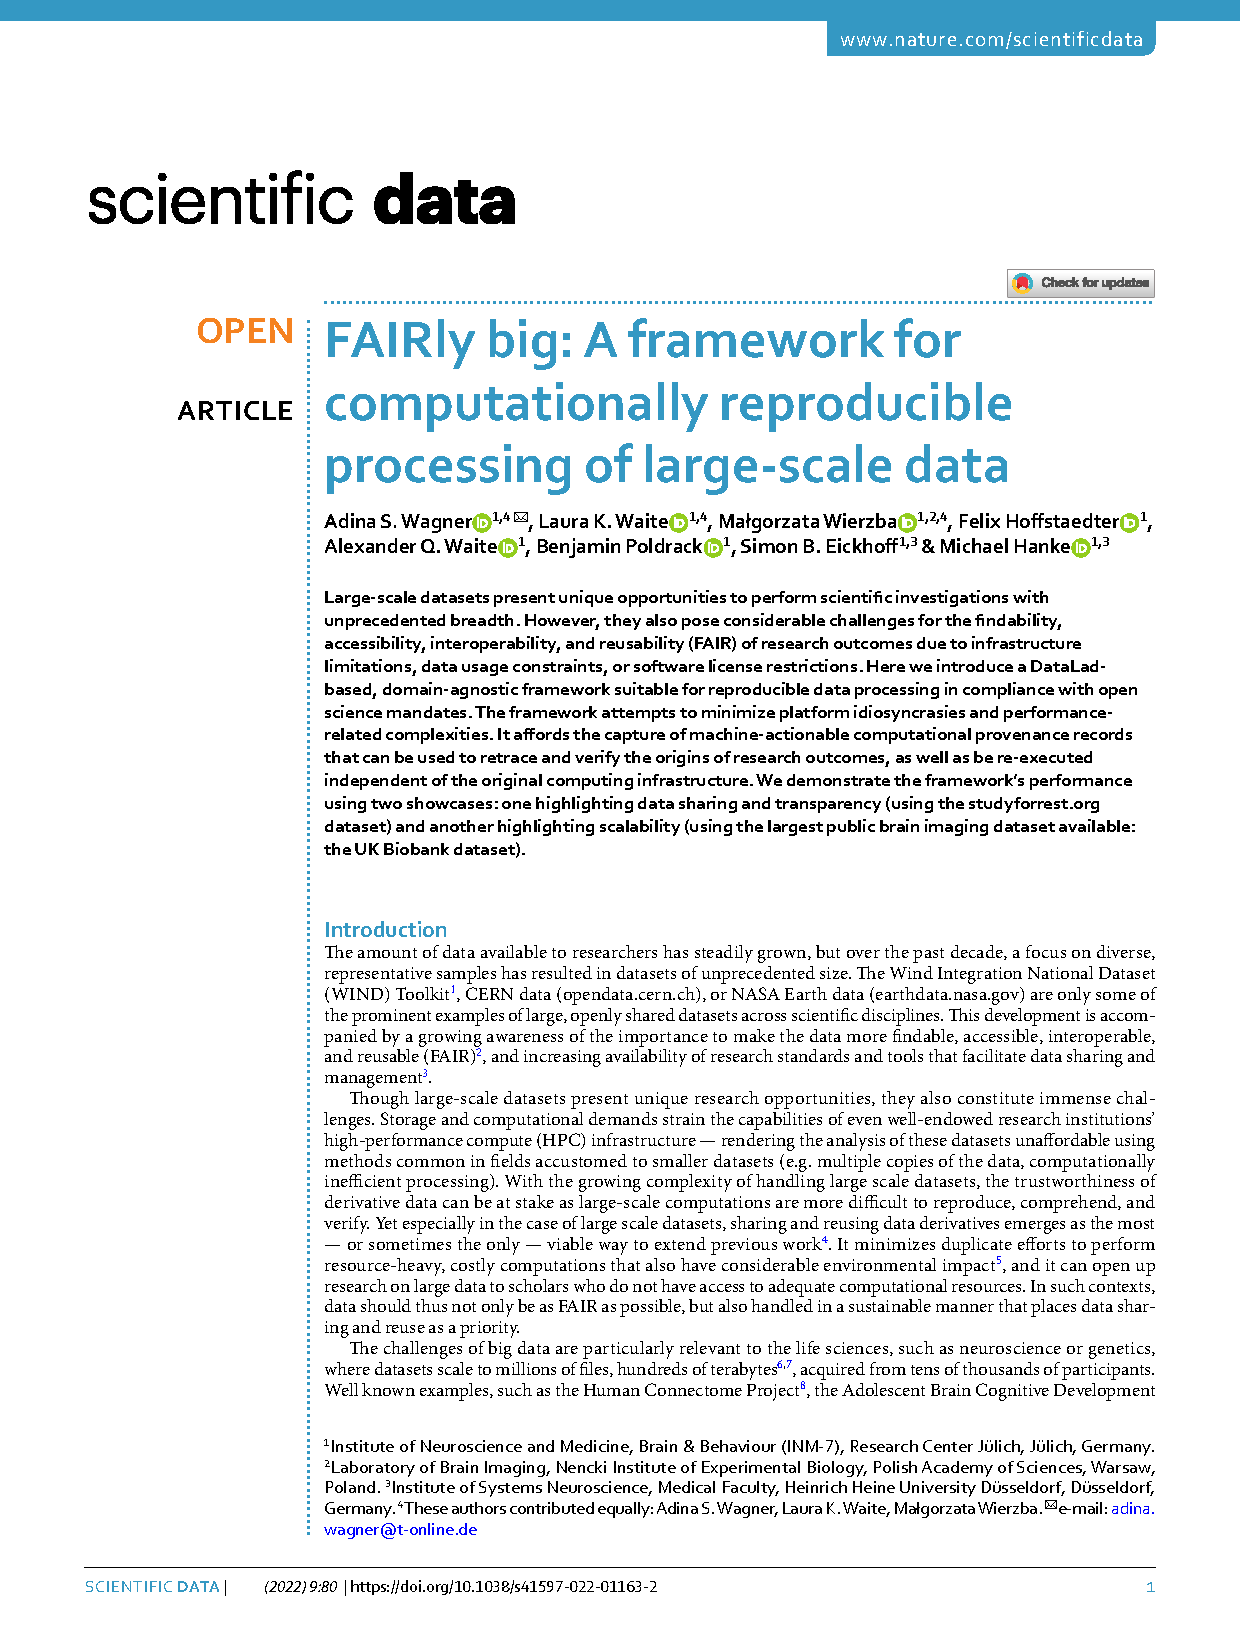
\includepdf[pages=1-17]{content/appendix_pub_fairlybig.pdf}
\includepdf[pages=1-8]{content/appendix_pub_datalad.pdf}

\end{refsection}
%

%\input{latexhints-english}

\pagestyle{empty}
\renewcommand*{\chapterpagestyle}{empty}
\Versicherung
\end{document}
